\section{Influence Propagation}
\label{sec:influ}

As we discussed in Section~\ref{sec:meth}, 
many files are submitted to VirusTotal more than once, 
and more than 99\% submissions are analyzed by at least 50 anti-virus engines. 
We observe that some engines fail to identify some malwares during early submissions, 
but they catch up when analyzing later submissions. 
Anti-virus vendors frequently use VirusTotal to identify false negatives in their products, 
which are malwares they fail to detect but detected by other vendors. 
We assume that there are influence among different anti-virus vendors.
In this section, we try to model this influence,
and try to predict whether an engine will identify a file as malware in the future, 
after the engine has already labeled the file as benign.

Influence propagation on social graph is a well-studied topic in web mining area. 
The static models we apply are proposed by~\citet{Influence} to analyze Flickr data.
We will first overview the static models~\cite{Influence} in our usage scenario in Section~\ref{sec:model}, 
and then we will discuss how to train models and use trained models to make prediction in Section~\ref{sec:predict}.  

\subsection{Influence Model}
\label{sec:model}


We assume that all vendors form a complete directed social graph $G = (V, E)$, 
where the nodes $V$ are vendors. 
The social graph is complete, 
since we assume there is possible influence from any vendor to all other vendors.
We assume there are action logs generated, 
when VirusTotal applies a set of anti-virus engines to analyze a submission. 
For each engine, there will be an action log $(u, a, t)$ or an action log $(u, \bar{a}, t)$, 
representing whether or not $u$ takes action to identify the submission as a malware at time $t$. 
To make things easy, after a vendor $u$ labels a file as malware, 
we assume $u$ will insist its decision, 
and ignore cases where a vendor labels a file as malware, but labels the file as benign later. 

We use $A_u$ to represent the number of actions taking by u, 
or the number of malwares identified by $u$. 
We use $\bar{A}_u$ to represent the number of malwares ever analyzed and labeled as benign by $u$.
We use $A_{u\&v}$ to represent the number of actions taken by both $u$ and $v$, 
and $A_{u|v}$ to represent the number of actions taken by either $u$ or $v$.
Clearly, $A_{u|v} =   A_u + A_v - A_{u\&v}$
We use $A_{u2v}$ to represent the number of actions propagated from $u$ to $v$. 
We define action propagation as follows: 

\begin{definition}{Action Propagation:}
We say that an action $a$ propagated from $u$ to $v$ iff: (i) $\exists$ $(v, \bar{a}, t_i)$ $\in$ $\bar{A}_v$, 
and $(v, a, t_k)$ $\in$ $A_v$, with $t_i < t_k$; (ii) $\exists$ $(u, a, t_j)$ $\in$ $A_u$, with $t_j < t_k$. 
\end{definition}

For each edge $(u, v) \in E$ in the social graph $G$, 
there is an influence probability: $p_{u,v}$,
which represent after $u$ takes an action the probability that $v$ will follow $u$ to take the same action. 
Since social graph $G$ is a complete graph, 
all other nodes are all $v$'s neighbors. 
For an action $a$, we use $S_v(a)$ to represent the set of $v$'s neighbors taking action $a$ before v. 
The probability that $v$ will follow its neighbors to take the same action is calculated as:

$$p_v(S_v(a)) = 1 - \prod\limits_{u \in S_v(a)}(1 - p_{u,v})$$

During training stage, we try to learn $p_{u,v}$ for each edge. 
During prediction stage, we provide a tunable threshold $\theta$. 
For node $v$ without taking an action $a$, 
if $P_v(S_v(a))>\theta$, 
we predict $v$ will follow its neighbors to take the action $a$ in the future. 

There are four static models, and they differ in how to estimate $p_{u,v}$. 

{\bf Bernoulli distribution.} $p_{u,v}$ is estimated as the ratio of the number of actions 
propagated from $u$ to $v$ over the total number of actions taken by $u$.

$$p_{u,v} = \frac{A_{u2v}}{A_u}$$ 

{\bf Jaccard index.} 
$p_{u,v}$ is estimated by the number of actions propagated from $u$ to $v$ dividing 
the number of actions taken either by $u$ or by $v$.

$$p_{u,v} = \frac{A_{u2v}}{A_{u|v}}$$ 

When $v$ takes an action $a$, it may be influenced by the combination of all its neighbors $S_v(a)$ 
taking the action $a$ before $v$. Partial credit takes this intuition. 
Partial credit for $u$ who takes an action $a$ before $v$ is calculated as:

$$credit_{u,v}(a) = \frac{1}{|S_v(a)|}$$

{\bf Bernoulli distribution with partial credit.} 
$p_{u,v}$ is estimated by the sum of all partial credits taking by $u$ for actions propagated from $u$ to $v$, 
dividing by the number of actions taken by $u$. 

$$p_{u,v} = \frac{\sum\limits_{a \in A_{u2v}}{credit_{u,v}(a)}}{A_v}$$

{\bf Jaccard index with partial credit.} 
$p_{u,v}$ is estimated by the sum of all partial credits taking by $u$ for actions propagated from $u$ to $v$, 
dividing by the number of actions taken either by $u$ or by $v$. 

$$p_{u,v} = \frac{\sum\limits_{a \in A_{u2v}}{credit_{u,v}(a)}}{A_v}$$




\subsection{Model Evaluation}
\label{sec:predict}

We split all PE submissions we collect into training set and testing set, based on submitted files’ sha256. 
If a sha256 starts with a numeric character, 
from ‘0’ to ‘9’, we will put its related submissions to training set, 
otherwise, we will put its related submissions to testing set.  
For a submitted file, all its submissions are put together either in training set or in testing set. 

The training process is implemented by several stages of map, filter, and reduce. 
We first reduce submission records according to submitted files. 
We sort submission records for each file chronologically, 
and filter out files without action propagation. 
For each file, we compute 4 maps based on its submission records. 
One map is one dimension, and it contains the number of actions taken by each vendor $u$. 
The other three maps are two dimension, and they contain an entry for each pair of vendors $(u,v)$, 
representing actions taken by both $u$ and $v$, actions propagated from $u$ to $v$, 
and partial credits taken by $u$ for actions propagated from $u$ to $v$. 
In the final reduce stage, 
we combine content of these 4 maps from different files, and calculate $p_{u,v}$ for the four models. 

After training 4 static models, we filter out engines taking less than 10000 actions,
because we think for engines taking too few actions, results may not be reliable. 
As a result, we have 59 engines left. 
For confidential reasons, we omit vendors’ name in the following discussion, 
and use number 0 - 58 to represent each engine. 

For each static model, 
we put all learned $p_{u,v}$ in a table, 
by using $u$ as row number and $v$ as column number.
For any $p_{u,v}$, bernoulli distribution has the largest value, 
jaccard index has the second largest value, 
bernoulli with partial credit has the third largest value,
and jaccard index with partial credit has the least value. 

\begin{figure*}
\centering
\subfloat[]{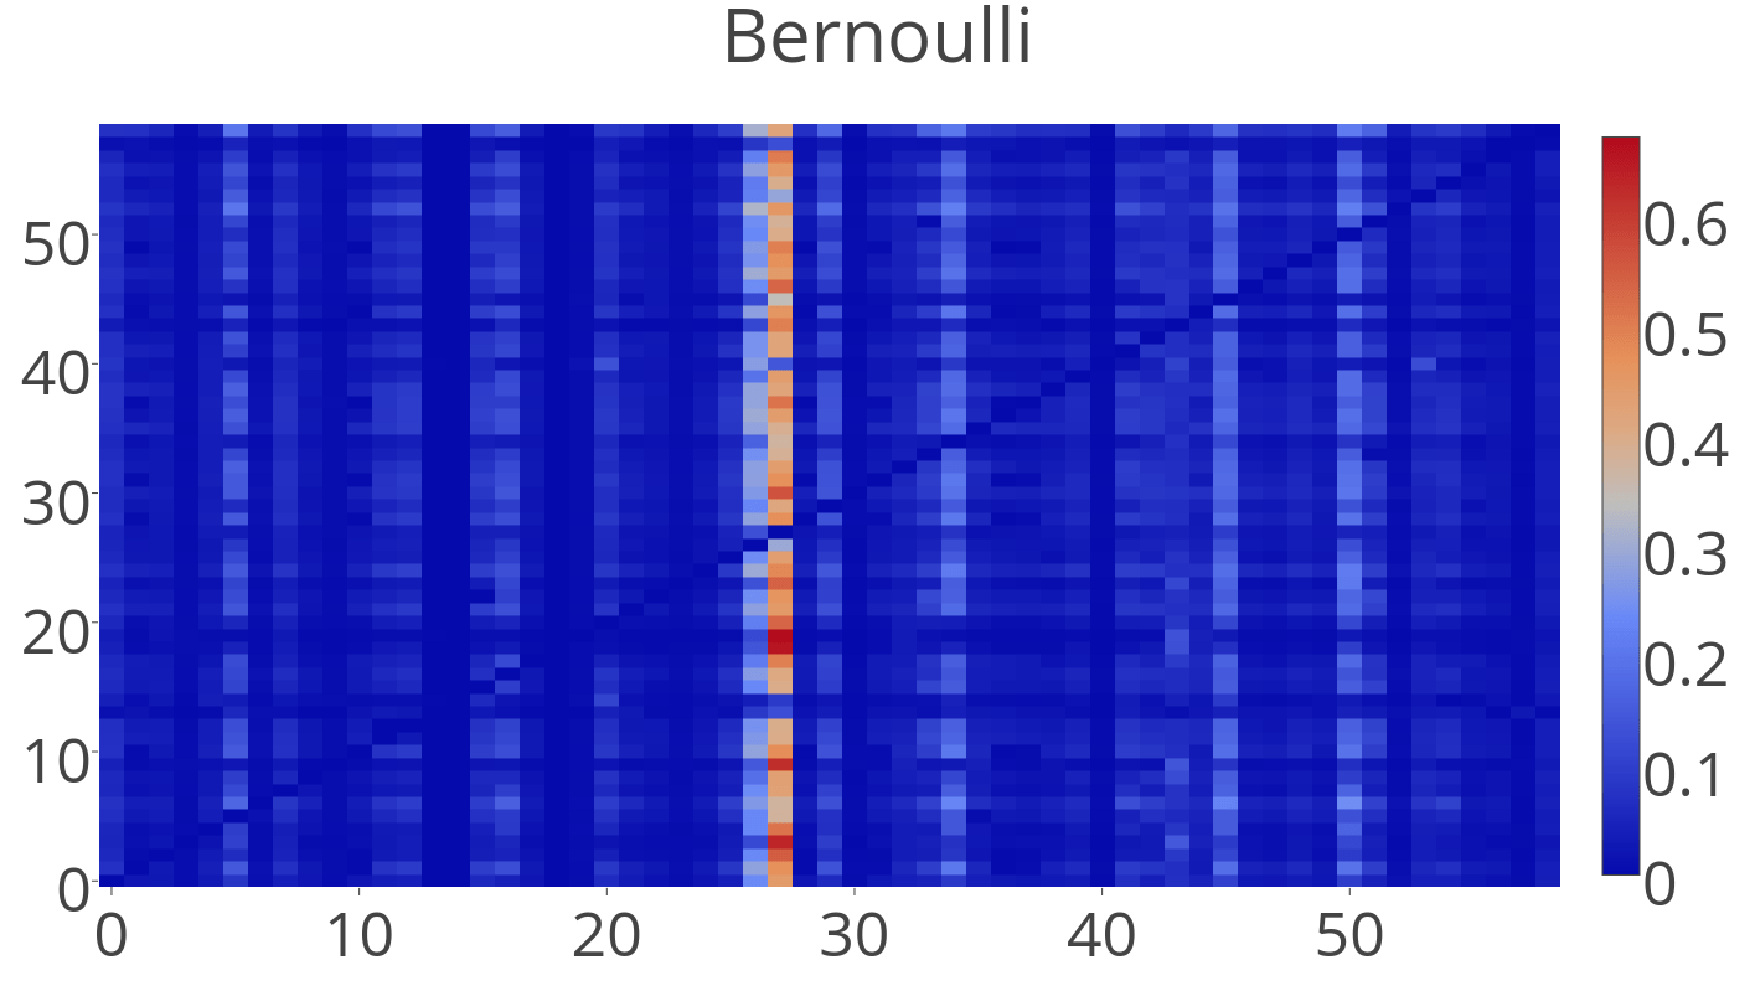
\includegraphics[width=0.24\linewidth]{figure/bernoulli-train}\label{fig:moredata1}} 
\subfloat[]{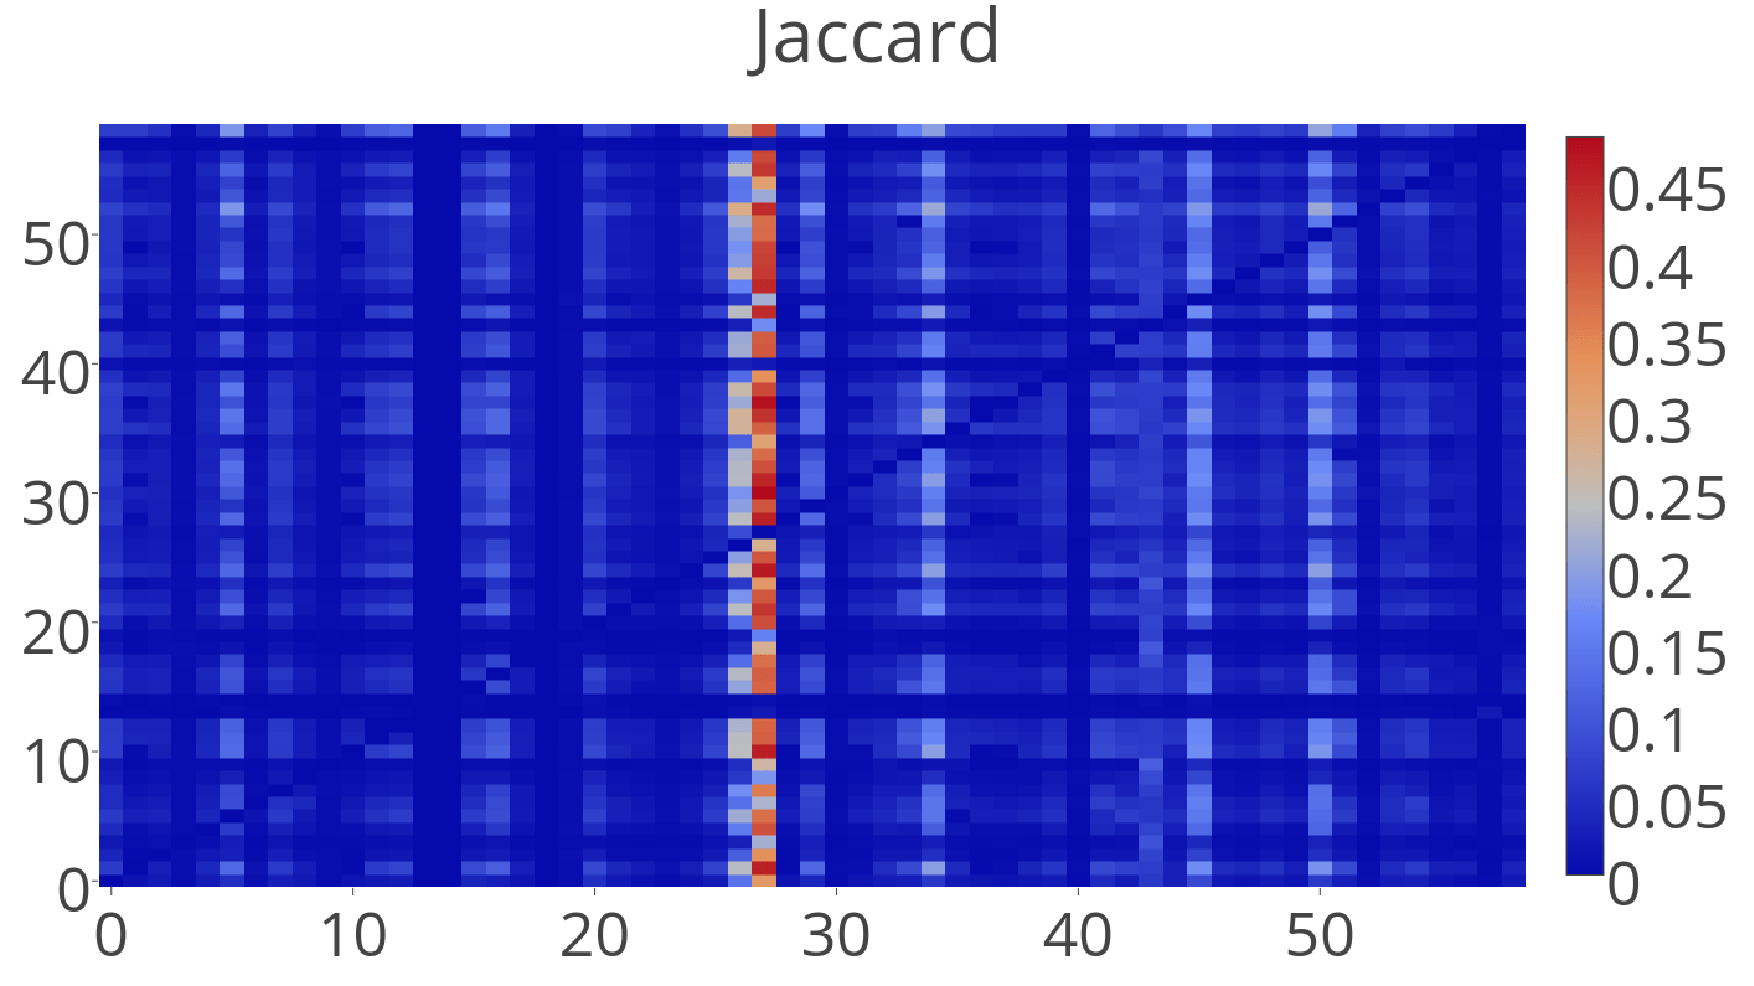
\includegraphics[width=0.24\linewidth]{figure/jaccard-train}\label{fig:moredata2}}
\subfloat[]{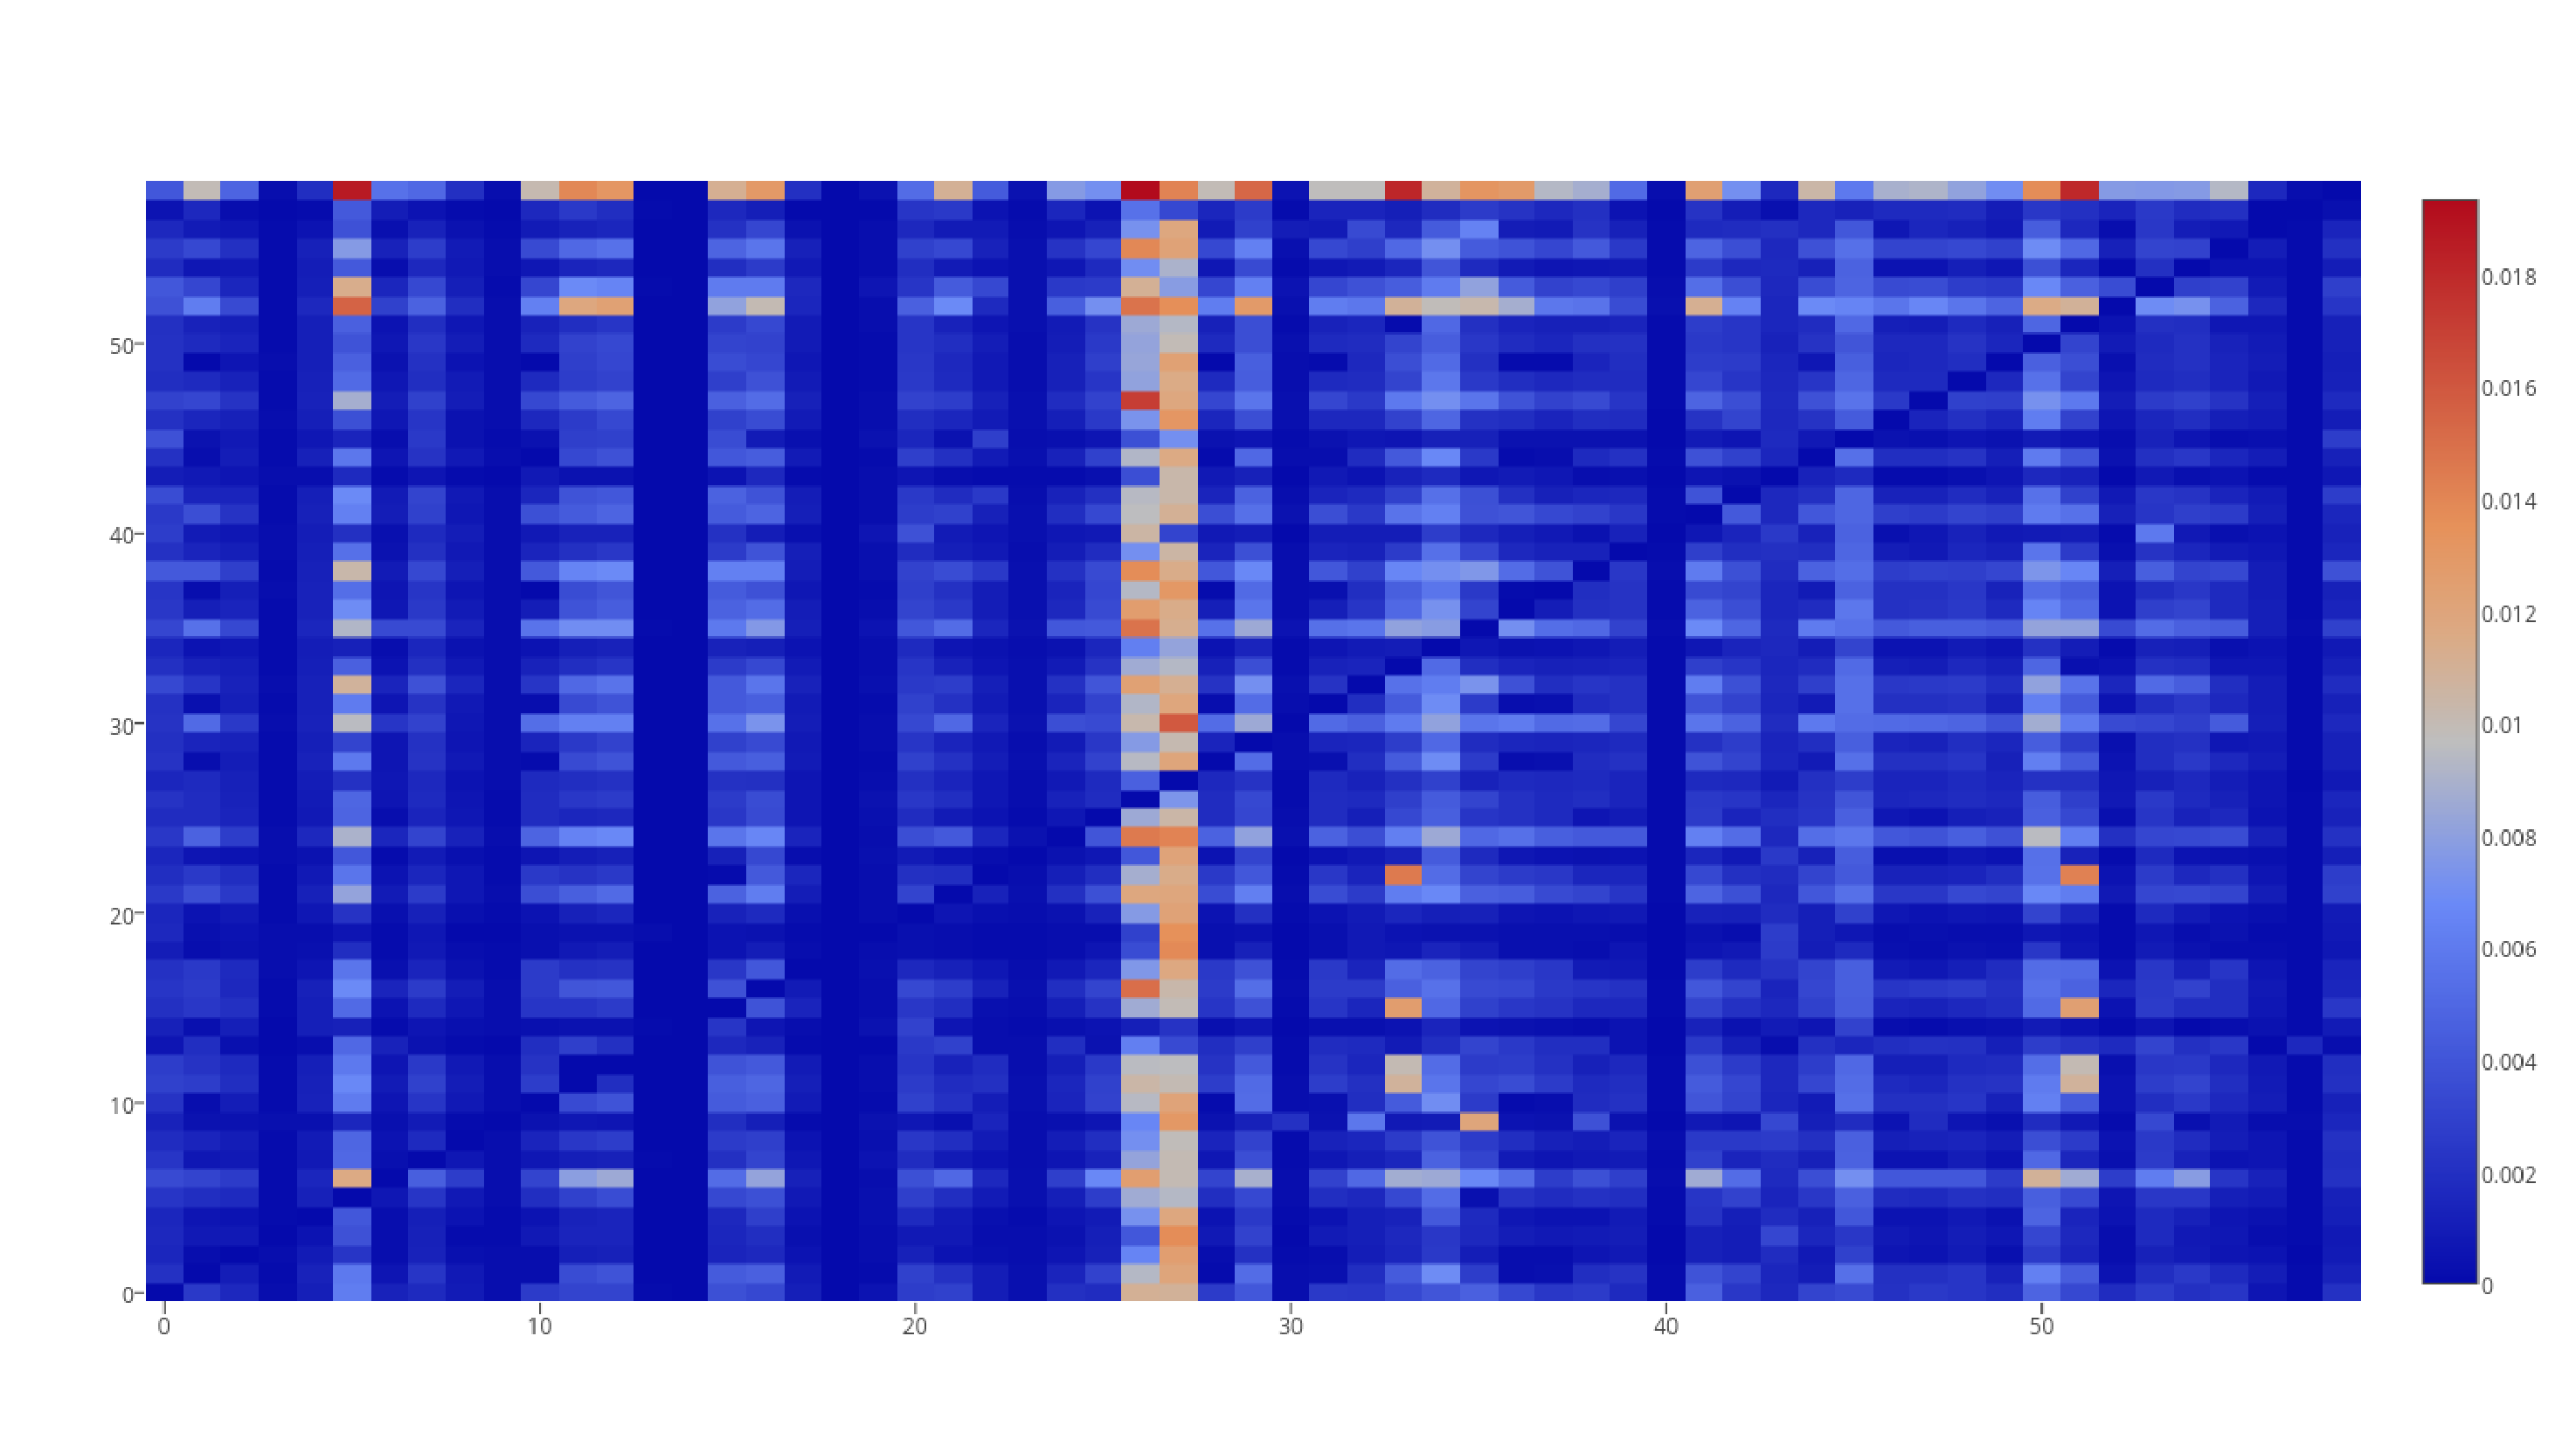
\includegraphics[width=0.24\linewidth]{figure/PC-train}\label{fig:moredata3}} 
\subfloat[]{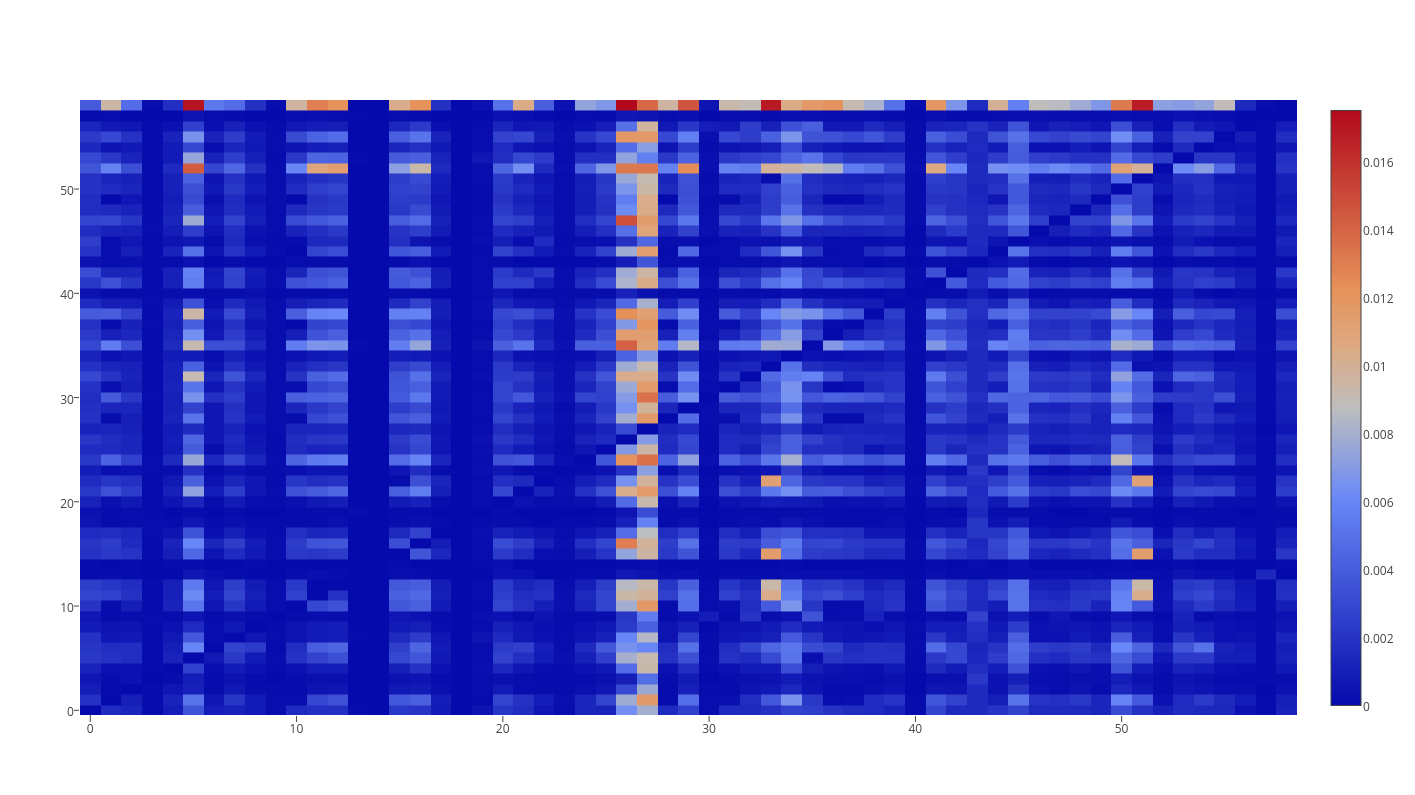
\includegraphics[width=0.24\linewidth]{figure/jaccardPC-train}\label{fig:moredata4}} \\ 
\caption{Potential for 0.5 V bias.} 
\label{fig:EcUND} 
\end{figure*} 


\begin{figure}[t!]
\begin{center}
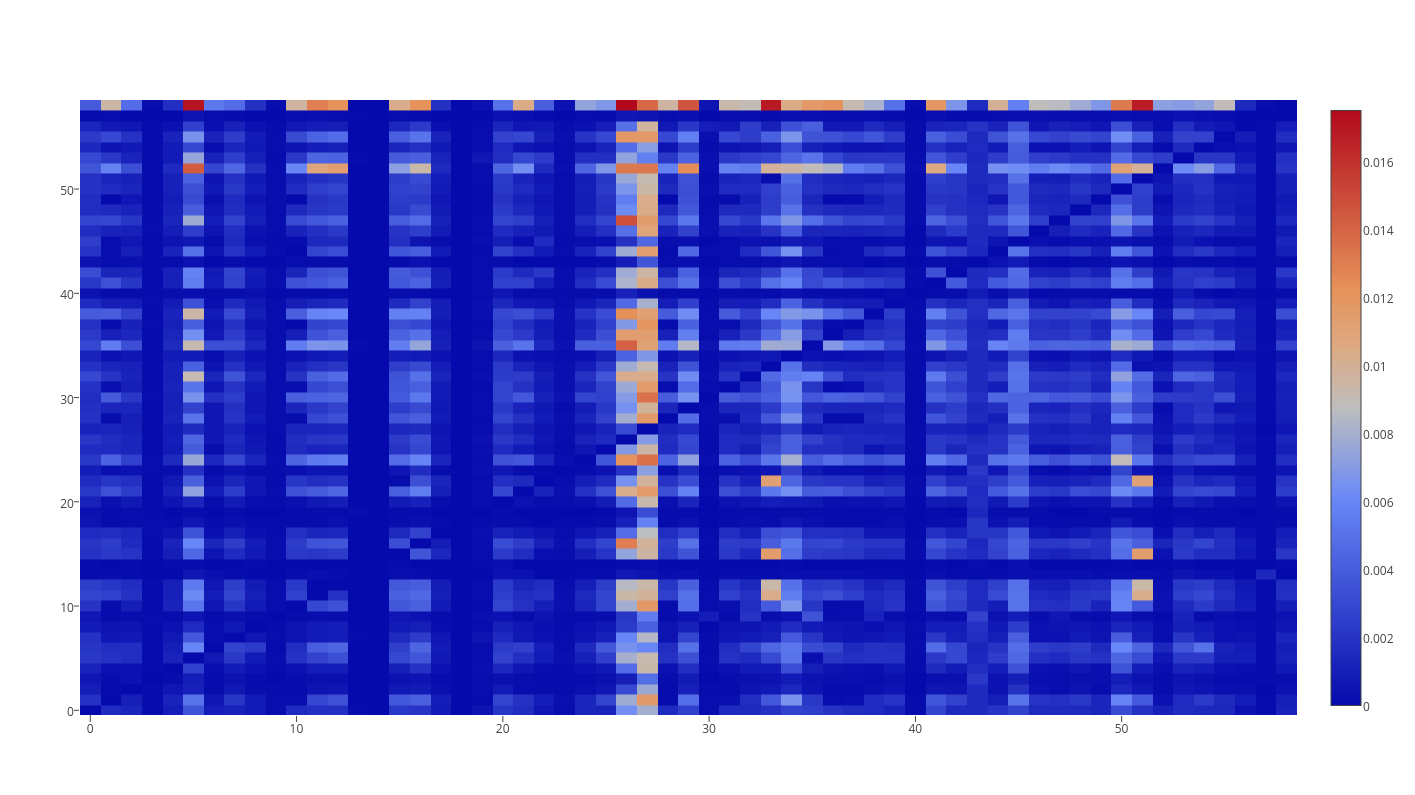
\includegraphics[width=2.5in]{figure/jaccardPC-train}
\mycaption{fig:idreputation}{Test.}
{\footnotesize{(How detection rate changes with the value of source id's reputation. Each reputation is rounded up to nearest 0.05.
Reputation -1 means the source id did not make any submission before. 95\% confidence interval is also drawn 
for each point.)}}
\end{center}
%\vspace{-0.25in}
\end{figure}

We draw heat maps for all tables in Figure~\ref{fig:heat}. 
Given a cell(u, v), red color means more influence from u to v. 
The four heat maps share a similar pattern.
From Figure~\ref{fig:heat}, 
we can see that there are no vendors which can influence all other vendors, 
but there are vendors which seem be influenced by all other vendors.  

We sum all numbers in a row together for each influence table. 
The results show how engine' influence rank in malware detection community. 
Same as heat maps, influence rankings also share a similar pattern. 

The test process is also implemented by several stages of map, filter, and reduce. 
Same as what we did during training, 
we filter out submitted files without action propagations, 
and sort submissions for left files chronologically. 
Given a submission, we calculate $p_v(S_v(a))$ for each engine $v$, 
which labeled the submitted file as benign before, but have not labeled the file as malware. 
$S$ is the set of engines which have already labeled the file as malwares.
We compare $p_v(S_v(a))$ with a given threshold to decide whether we will predict 
$v$ will label the file as malware. We count true positive (TP), false positive (FP), true negative (TN), 
and false negative (FN), by comparing our prediction with engines' real actions. 
In the final stage, we reduce TP, TN, FP, and FN numbers from different files.


\begin{figure}[t!]
\begin{center}
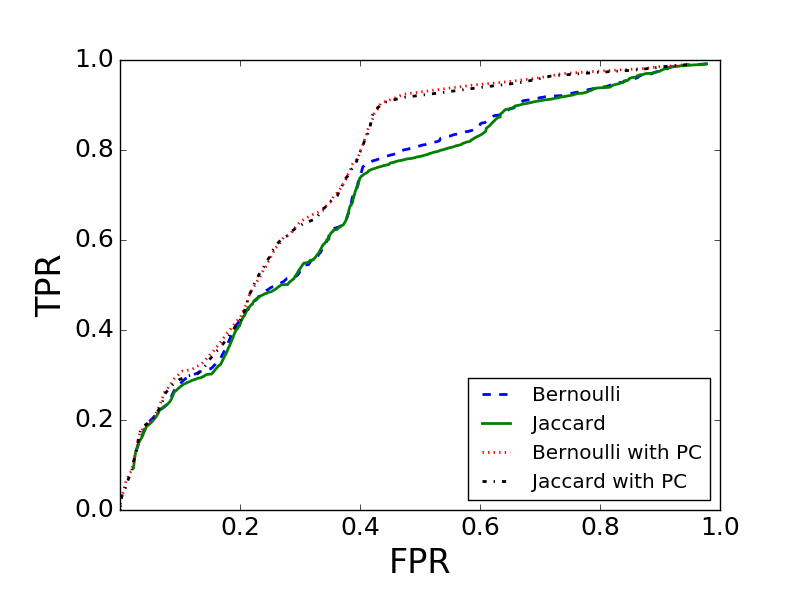
\includegraphics[width=2in]{figure/predict}
\vspace{-0.1in}
\caption{ROC comparisons of Static Models. 
(How true positive rate (TPR) changes with false positive rate (FPR). 
We change probability threshold from 0.1\% to 99.9\% with step 0.1\%. 
We compute TPR and FPR for each probability threshold to draw the curve.)
}
\label{fig:predict}
\end{center}
\vspace{-0.1in}
\end{figure}

We change the probability threshold from 0.1\% to 99.9\%, by using 0.1\% as step. 
We depict the performance of static models by using ROC curves, 
with true positive rate ($TPR = TP/(TP+FN)$) as x-axis, 
and false positive rate (FPR = FP/(FP + FN)) as y-axis. 
ROC curves for the 4 static models are shown in Figure~\ref{fig:predict}. 
The closer the hump of the ROC curve to $(0,1)$, the better performance.
Bernoulli with partial credit is as good as jaccard index, 
and both of them are better than bernoulli and jaccard index. 


\subsection{Discussion}

There are also time models proposed by ~\citet{Influence}. 
Time information we have is when a submission is conducted, or when an engine analyzes a submission. 
Although we can obverse detection result change from submission sequence, 
submission time is different from when engines change their detection results. 

Our data collection ends on 09/06/2016. 
There could be cases where we predict engines will change their results, 
engines have not change right now, but will change in the future.  
We think prediction results we present are conservative. 

End users can use our results to pick up good anti-virus products. 
Security experts know which engines’ results are more trustable. 
Vendors can identify possible false positive and false negatives in their products. 